\documentclass[00_complete]{subfiles}

%\documentclass[12pt]{report}
\usepackage[utf8]{inputenc}
\usepackage{amsmath,amssymb,amsthm,gensymb,parskip,graphicx,footmisc,csquotes,enumerate,datetime2}
\usepackage[]{libertinus}
\usepackage[breaklinks]{hyperref}
\hypersetup{
  pdfauthor={Moshe Krumbein},
  colorlinks=true,
  linkcolor={black},
  filecolor={black},
  citecolor={black}, %blue
  urlcolor={black}, %blue
}
\usepackage[top=30mm,bottom=30mm,left=30mm,right=30mm]{geometry}
%\setlength{\emergencystretch}{2em} % prevent overfull lines
\providecommand{\tightlist}{%
\setlength{\itemsep}{0pt}\setlength{\parskip}{0pt}}

\renewcommand\qedsymbol{$\blacksquare$}

\theoremstyle{definition}
\newtheorem*{definition}{Definition}
\newtheorem*{theorem}{Theorem}
\newtheorem*{axiom}{Axiom}
\newtheorem*{lemma}{Lemma}

\theoremstyle{remark}
\newtheorem*{note}{Note}
\newtheorem*{symbols}{Symbol}
\newtheorem{example}{Example}[section]
\newtheorem*{claim}{Claim}
\newtheorem*{conclusion}{Conclusion}
\newtheorem*{reminder}{Reminder}

\usepackage{fancyhdr}
\usepackage[italicdiff]{physics}
\MakeOuterQuote{"}

\renewcommand{\chaptermark}[1]{\markboth{#1}{}}

\pagestyle{fancy}

\setlength{\headheight}{14.5pt}
\addtolength{\topmargin}{-2.5pt}

\fancyhf{}
\rhead{Moshe Krumbein}
\lhead{\chaptermark}
\cfoot{\thepage}
\fancyhead[R]{\chaptername~\thechapter}
\fancyhead[L]{\mbox{\leftmark}}

\usepackage[Rejne]{fncychap}
\usepackage{titling}

\makeatletter
\renewcommand{\@chapapp}{\vspace*{-100pt}\huge\thetitle}
\makeatother

\makeatletter
\newcommand{\subtitle}[1]{%
  {\center\vspace*{-60pt}%
  \linespread{1.1}\Large\scshape#1%
  \par\nobreak\vspace*{35pt}}
}
\makeatother

\newcommand{\Chapter}[2]{
    \def\n{#2}
    \setcounter{chapter}{\the\numexpr\n-1}
    \chapter{#1}
    \subtitle{\theauthor~- \thedate}
}

\DeclareMathOperator{\Ima}{Im}
\DeclareMathOperator{\Id}{Id}
\DeclareMathOperator{\cis}{cis}

\newcommand{\Mod}[1]{\ (\mathrm{mod}\ #1)}
\newcommand{\st}[0]{\;\mathrm{s.t.}\;}

\title{Discrete Mathematics}
\author{Moshe Krumbein}
\date{Fall 2021}

\begin{document}
\Chapter{Partial Ordered Relations}{4}

\section{Partial Ordered Relations}

Given relation \(R\) on a set, then we say the \(R\) is a partial ordered
relation if \(R\) is \emph{reflexive}, \emph{antisymmetric}, and
\emph{transitive}. In this case we say that \(A\) is a \emph{partial ordered
set}.

\begin{definition}
A partial ordered relation that exists for all
\(\forall \: x,y \in R \;\exists\; (x,y) \in R\) or \((y,x) \in R\) is
called a \emph{linear order}.
\end{definition}

Suppose that \(R\) is a partial ordered relation on \(A\):
\[(a,b) \in R \quad a \leq_R b\]

\(x \in A\) is called the \emph{maximum} if \(\forall \; y \in A\), if
\((x,y) \in R\), then \(x=y\). (\(x\) has no arrows going out of it
except for to itself).

\(x \in A\) is called the \emph{minimum} if \(\forall \; y \in A\), if
\((y,x) \in R\), then \(x=y\). (\(x\) has no arrows going to it except
for to itself).

\section{\href{https://en.wikipedia.org/wiki/Hasse_diagram}{Hasse
Diagram}}

We'll say that pair \((x,y) \in R\) is "required" in a Hasse diagram
if \(x \neq y\), and therefore:
\[\forall z \in A (x,z),(z,y) \in R \implies z=x \text{ or } z=y\]

Essentially, we can get rid of all arrows that represent transitivity and
reflexivity because they are assumed.

\begin{figure}[ht!]
    \centering
    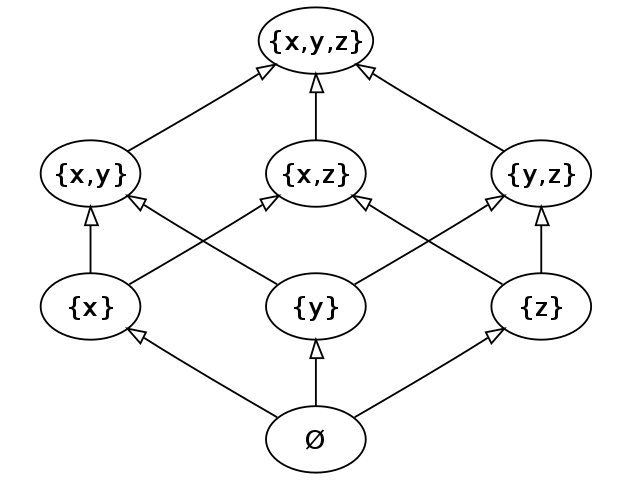
\includegraphics[width=0.5\textwidth]{w4-hesse}
    \caption{Example of a Hesse diagram}
\end{figure}

\begin{claim}
If \(R\) is a linear ordered relation on \(A\) then there exists in
\(A\) only one maximum and minimum.
\end{claim}
\end{document}
